% =============================================================================
% Project : THE_PHILOSOPHY_OF_VIABILITY
% Book    : Book I — Ontology of Viability
% Book ID : VS.B01
%
% File    : 4_ASSETS/illustrations/VS.B01.P01.C03.S03.SS09.P009.IL01.common_origin_and_aggregate_grouping.tex
%
% Asset   : IL01 — Common Origin and Aggregate Grouping
%
% Purpose :
%   To illustrate the distinction between a common productive
%   source and unity established through the grouping of elements.
%
% Illustration Policy :
%   The example clarifies two different relations. It does not
%   establish the identity, numerical unity, or ontological status
%   of the objects, their producers, or the resulting collection.
%
% Requires (preamble):
%   \usepackage{tikz}
% =============================================================================

\begin{figure}[htbp]
    \centering

    % distance between panel centres (panel width 5.8 cm + gap 0.4 cm)
    \def\pw{6.2}

    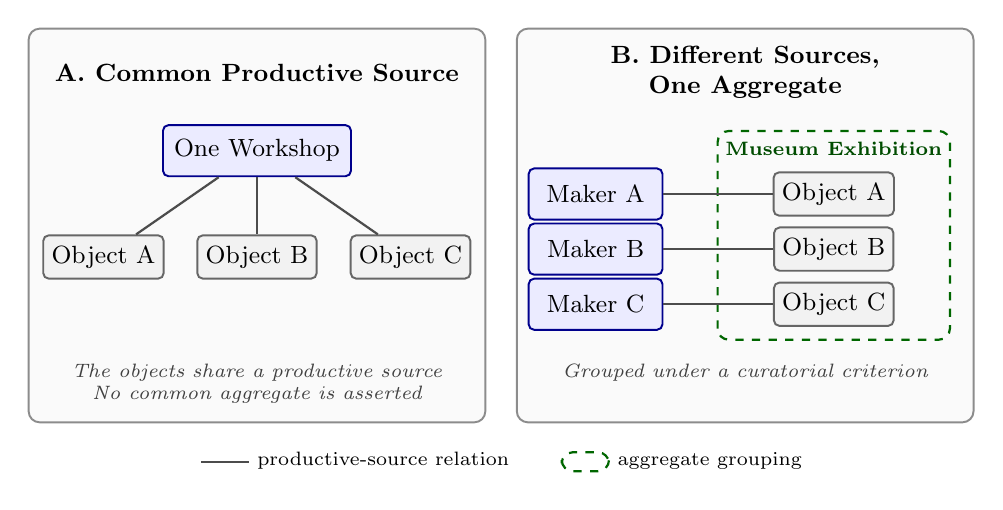
\begin{tikzpicture}[
        font=\small,
        % --- panel, title, note ---
        panel/.style={draw=black!45, fill=gray!4, rounded corners=4pt,
                      line width=0.7pt},
        ptitle/.style={font=\small\bfseries, align=center, text width=5.3cm,
                       minimum height=0.9cm, anchor=north, inner sep=0pt},
        pnote/.style={font=\scriptsize\itshape, text=black!75, align=center,
                      text width=5.3cm, anchor=north, inner sep=0pt},
        % --- node roles ---
        src/.style={draw=blue!55!black, fill=blue!8, rounded corners=2pt,
                    align=center, minimum width=2.2cm, minimum height=0.65cm,
                    inner sep=4pt, line width=0.7pt},
        elem/.style={draw=black!60, fill=gray!10, rounded corners=2pt,
                     align=center, minimum width=1.5cm, minimum height=0.55cm,
                     inner sep=3pt, line width=0.7pt},
        % --- aggregate: dashed green frame (as in DG01, C03.S03.SS07) ---
        aggregate/.style={draw=green!40!black, dashed, rounded corners=4pt,
                          line width=0.8pt},
        aglabel/.style={font=\scriptsize\bfseries, text=green!30!black},
        % --- productive-source relation (undirected: no arrowheads) ---
        srcrel/.style={draw=black!70, line width=0.8pt}
    ]

    % ---------------------------------------------------------------
    % Panel A — common productive source
    % ---------------------------------------------------------------
    \begin{scope}
        \draw[panel] (-2.9,-2.5) rectangle (2.9,2.5);
        \node[ptitle] at (0,2.4) {A. Common Productive Source};

        \node[src] (w) at (0,0.95) {One Workshop};
        \node[elem] (oa) at (-1.95,-0.4) {Object A};
        \node[elem] (ob) at (0,-0.4)     {Object B};
        \node[elem] (oc) at (1.95,-0.4)  {Object C};

        \draw[srcrel] (w) -- (oa);
        \draw[srcrel] (w) -- (ob);
        \draw[srcrel] (w) -- (oc);

        \node[pnote] at (0,-1.75) {
            The objects share a productive source\\
            No common aggregate is asserted
        };
    \end{scope}

    % ---------------------------------------------------------------
    % Panel B — different sources, one curatorial aggregate
    % ---------------------------------------------------------------
    \begin{scope}[shift={(\pw,0)}]
        \draw[panel] (-2.9,-2.5) rectangle (2.9,2.5);
        \node[ptitle] at (0,2.4) {B. Different Sources, One Aggregate};

        % aggregate frame (drawn first, so its content sits on top)
        \draw[aggregate] (-0.35,-1.45) rectangle (2.6,1.2);
        \node[aglabel] at (1.125,0.98) {Museum Exhibition};

        \node[src, minimum width=1.7cm] (ma) at (-1.9,0.4)  {Maker A};
        \node[src, minimum width=1.7cm] (mb) at (-1.9,-0.3) {Maker B};
        \node[src, minimum width=1.7cm] (mc) at (-1.9,-1.0) {Maker C};

        \node[elem] (ea) at (1.125,0.4)  {Object A};
        \node[elem] (eb) at (1.125,-0.3) {Object B};
        \node[elem] (ec) at (1.125,-1.0) {Object C};

        \draw[srcrel] (ma.east) -- (ea.west);
        \draw[srcrel] (mb.east) -- (eb.west);
        \draw[srcrel] (mc.east) -- (ec.west);

        \node[pnote] at (0,-1.75) {Grouped under a curatorial criterion};
    \end{scope}

    % ---------------------------------------------------------------
    % Legend
    % ---------------------------------------------------------------
    \node[font=\scriptsize] at ({\pw/2},-3.0) {
        \tikz[baseline=-0.5ex]\draw[srcrel] (0,0) -- (0.6,0);~productive-source relation
        \quad\quad
        \tikz[baseline=-0.5ex]\draw[aggregate] (0,-0.12) rectangle (0.6,0.12);~aggregate grouping
    };

    \end{tikzpicture}

    \caption{Common Productive Origin and Unity Through Aggregate Grouping}
    \label{fig:common-origin-and-aggregate-grouping}
\end{figure}

% =============================================================================
% END OF ASSET IL01
% =============================================================================